% Mirror: https://github.com/SIGma-UIUC/presentation-format
% --------------------------------------------------------------------
% This is a simple Beamer document that uses beamerthemesigma.sty
% Reading the comments should help you create a presentation even if
% you've never used Beamer before.
% --------------------------------------------------------------------

% Set our document class to Beamer
\documentclass[aspectratio=169]{beamer}

% Some packages for nice font encodings in the final PDF
\usepackage[utf8]{inputenc}
\usepackage[T1]{fontenc}

\usepackage{tikz}

% From Jeff E
\usepackage{algo}

% Some more macros
\usepackage{sigmastyle}

% Citations
\usepackage{cite}

% To insert images
\usepackage{graphicx}

% Useful packages from the AMS
\usepackage{amsmath,amssymb,amsthm}

\usepackage{soul}

% Package for code highlighting
\usepackage{minted}
\setminted{linenos=true, breaklines=true, breakanywhere=true, style=default}
\usemintedstyle{monokai}

% Set a title
\title{Generating Permutations}

% Set a subtitle if you desire
\subtitle{\cite[Chapter~7.2.1.2]{TAOCP4A}}

% Whoever worked on the presentation:
\author{Sam Ruggerio}

% Date looks ugly, so leave blank
\date{}

% An institute name, if you're so inclined
% \institute{University of Illinois Urbana-Champaign}

% Use the SIGma theme for this Beamer presentation
\usetheme{sigma}
% --------------------------------------------------------------------

% Begin document
\begin{document}

% Beamer calls each slide a "frame", defined within the environment:
% \begin{frame}
%   <frame content here>
% \end{frame}

% This frame is just the title.
\begin{frame}
\titlepage
\end{frame}

% A frame with the table of contents.
% This frame's title is "Outline".
\begin{frame}{Outline}
  \tableofcontents
\end{frame}

% \begin{frame}{Updates!}
%   % Let's put some real content in this frame:
%   Weekly updates:
%   \begin{itemize}
%     \item SIGma is an excellent SIG.
%     \item I'm out of ideas for updates.
%   \end{itemize}
% \end{frame}

% Start a section: *sections* (subsections, etc.) are what show up in the TOC.
\section{Permutations}

\frame{\sectionpage}

\begin{frame}{What is a Permutation}
\begin{itemize}
    \item Given a (multi)set $S$ a permutation is an \textcolor{sigma@mainblue}{ordered} sequence of every item in $S$ \pause
    \begin{itemize}
        \item A set is an unordered collection of distinct items
        \item A multiset allows repeated items \pause
    \end{itemize}
    \item For $n$ elements there are $n!$ possible permutations \pause
    \begin{itemize}
        \item $n$ possibilities for the first item... $n-1$ for the second... so on
    \end{itemize}
\end{itemize}
\end{frame}

\begin{frame}{Enumerating Permutations}
\begin{itemize}
    \item No surprises here, algorithms to enumerate permutations are going to require $O(n!)$ time \pause
    \item It's nice if algorithms output permutations in either 
    \begin{enumerate}[(a)]
        \item Some sorted order (lexographic)
        \item Minimal change between permutations (Gray) \pause
    \end{enumerate}
    \item Our algorithm will be slow in it's entirety, but we want to minimize "delay" between outputs. 
    \begin{itemize}
        \item We want to achieve $O(1)$ delay between permutations
    \end{itemize}
\end{itemize}
\end{frame}

\section{Algorithm L}
\frame{\sectionpage}

\begin{frame}{Lexographic Permutation}
\begin{itemize}
    \item A lexographic permutation of the multiset \{1,2,2,3\}:
\end{itemize}
\begin{table}[]
\begin{tabular}{llll}
1223 & 1232 & 1322 & 2123 \\
2132 & 2213 & 2231 & 2312 \\
2321 & 3122 & 3212 & 3221
\end{tabular}
\end{table} \pause
\begin{itemize}
    \item Let's assume we start a sequence $\{a_1, \dots, a_n\}$ that is sorted, such that $a_1 \leq a_2 \leq \cdots \leq a_n$
    \item We also insert a sentinel $a_0$ that's smaller than everything.
\end{itemize}
\end{frame}

\begin{frame}{Algorithm L}
\begin{nalgo}
\textul{\textbf{\textsc{AlgorithmL}}$(S[a_0, \dots, a_n])$}: 
\\\label{}  $j \gets n-1$
\\\label{}  \textbf{while} $j > 0$:\+ 
\\\label{}      \textsc{print}$(S)$ 
\\\label{}      $j \gets n-1$
\\\label{}      \textbf{while} $S[j] \geq S[j+1]$:\+
\\\label{}          decrement $j$\-
\\\label{}      \textbf{if} $j = 0$: \+
\\\label{}          continue \- 
\\\label{}      $l \gets n$ 
\\\label{}      \textbf{while} $S[j] \geq S[l]$ \+
\\\label{}          decrement $l$\-
\\\label{}      \textsc{swap}$(S[j], S[l])$
\\\label{}      \textsc{reverse}$(S, j+1, n)$
\end{nalgo}
\end{frame}

\begin{frame}{}
\begin{minipage}[c]{0.6\textwidth}
\begin{nalgo}
\textul{\textbf{\textsc{AlgorithmL}}$(S[a_0, \dots, a_n])$}: 
\\\label{}  $j \gets n-1$
\\\label{}  \textbf{while} $j > 0$:\+
\\\label{}      \textsc{print}$(S)$
\\\label{}{\color{lightgray}      $j \gets n-1$}
\\\label{}{\color{lightgray}      \textbf{while} $S[j] \geq S[j+1]$:\+}
\\\label{}{\color{lightgray}          decrement $j$\-}
\\\label{}{\color{lightgray}      \textbf{if} $j = 0$: \+}
\\\label{}{\color{lightgray}          continue \-}
\\\label{}{\color{lightgray}      $l \gets n$}
\\\label{}{\color{lightgray}      \textbf{while} $S[j] \geq S[l]$ \+}
\\\label{}{\color{lightgray}          decrement $l$\-}
\\\label{}{\color{lightgray}      \textsc{swap}$(S[j], S[l])$}
\\\label{}{\color{lightgray}      \textsc{reverse}$(S, j+1, n)$}
\end{nalgo}
\end{minipage}
\begin{minipage}[c]{0.35\textwidth}
\begin{itemize}
    \item If $j=0$, we've reached our sentinel value, and there's nothing left to permute \pause
    \item Otherwise, each iteration of this while loop will print out a permutation. 
\end{itemize}
\end{minipage}
\end{frame}

\begin{frame}{}
\begin{minipage}[c]{0.6\textwidth}
\begin{nalgo}
\textul{\textbf{\textsc{AlgorithmL}}$(S[a_0, \dots, a_n])$}: 
\\\label{}  $j \gets n-1$
\\\label{}  \textbf{while} $j > 0$:\+
\\\label{}      \textsc{print}$(S)$
\\\label{}      $j \gets n-1$
\\\label{}      \textbf{while} $S[j] \geq S[j+1]$:\+
\\\label{}          decrement $j$\-
\\\label{}      \textbf{if} $j = 0$: \+
\\\label{}          continue \-
\\\label{}      $l \gets n$
\\\label{}      \textbf{while} $S[j] \geq S[l]$ \+
\\\label{}          decrement $l$\-
\\\label{}      \textsc{swap}$(S[j], S[l])$
\\\label{}{\color{lightgray}      \textsc{reverse}$(S, j+1, n)$}
\end{nalgo}
\end{minipage}
\begin{minipage}[c]{0.35\textwidth}
\begin{itemize}
    \item We find the largest $j$ such that $a_j$ can be increased\pause
    \item Then, we find the smallest amount we can increase $a_j$ by (the search for $l$).
\end{itemize}
\end{minipage}
\end{frame}


\begin{frame}{}
\begin{minipage}[c]{0.6\textwidth}
\begin{nalgo}
\textul{\textbf{\textsc{AlgorithmL}}$(S[a_0, \dots, a_n])$}: 
\\\label{}{\color{lightgray}  $j \gets n-1$}
\\\label{}{\color{lightgray}  \textbf{while} $j > 0$:\+}
\\\label{}{\color{lightgray}      \textsc{print}$(S)$}
\\\label{}{\color{lightgray}      $j \gets n-1$}
\\\label{}{\color{lightgray}      \textbf{while} $S[j] \geq S[j+1]$:\+}
\\\label{}{\color{lightgray}          decrement $j$\-}
\\\label{}{\color{lightgray}      \textbf{if} $j = 0$: \+}
\\\label{}{\color{lightgray}          continue \-}
\\\label{}{\color{lightgray}      $l \gets n$}
\\\label{}{\color{lightgray}      \textbf{while} $S[j] \geq S[l]$ \+}
\\\label{}{\color{lightgray}          decrement $l$\-}
\\\label{}{\color{lightgray}      \textsc{swap}$(S[j], S[l])$}
\\\label{}     \textsc{reverse}$(S, j+1, n)$
\end{nalgo}
\end{minipage}
\begin{minipage}[c]{0.35\textwidth}
\begin{itemize}
    \item We've generated the prefix $a_1, \dots, a_j$, but the second half is now $a_n, \dots, a_{j+1}$, so we reverse it.
\end{itemize}
\end{minipage}
\end{frame}

% \begin{frame}{Algorithm L}
% \begin{algo}
% $j \gets n-1$ \\
% \textbf{while} $j > 0$:\+ \\
%     \textsc{print}$(S)$
% \end{algo}
% 
% \begin{itemize}
%     \item If $j=0$, we've reached our sentinel value, and there's nothing left to permute \pause
%     \item Otherwise, each iteration of this while loop will print out a permutation. 
% \end{itemize}
% \end{frame}

% \begin{frame}{Algorithm L}
% \begin{algo}
%     $j \gets n-1$ \\
%     \textbf{while} $S[j] \geq S[j+1]$:\+ \\
%     decrement $j$\- \\
%     \textbf{if} $j = 0$: \+ \\
%     continue \- \\
%     $l \gets n$ \\
%     \textbf{while} $S[j] \geq S[l]$: \+ \\
%     decrement $l$\- \\
%     \textsc{swap}$(S[j], S[l])$
% \end{algo}
% 
% \begin{itemize}
%     \item We find the largest $j$ such that $a_j$ can be increased\pause
%     \item Then, we find the smallest amount we can increase $a_j$ by (the search for $l$).
% \end{itemize}
% \end{frame}

% \begin{frame}{Algorithm L}
% \begin{algo}
%     \textsc{reverse}$(S, j+1, n)$
% \end{algo}
% 
% \begin{itemize}
%     \item We've generated the prefix $a_1, \dots, a_j$, but the second half is now $a_n, \dots, a_{j+1}$, so we need to reverse it.
% \end{itemize}
% \end{frame}

\begin{frame}{}
      \begin{center}
    {\color{sigma@mainblue} \LARGE Questions?}
  \end{center}
\end{frame}

\begin{frame}{Questions!}
\begin{itemize}
    \item What is the delay between permutations?
    \item What is (crudely) the runtime of this algorithm?
    \item If elements in $S$ are distinct, how often does the decrement $j$ step \textit{not} run?
\end{itemize}
\end{frame}

\section{Algorithm P}
\frame{\sectionpage}

\begin{frame}{Gray Permutation}
\begin{itemize}
    \item We want to generate permutations in a way so that only two adjacent elements swap at every iteration \pause
    \item This isn't guaranteed to happen in a multiset. \pause
    \begin{itemize}
        \item Consider a graph of permutations, where there are edges between adjacent swaps
        \item We want to find a Hamiltonian path, but multisets can generate graphs where there are none!
    \end{itemize}
\end{itemize}
\end{frame}

\begin{frame}{Gray Paths}
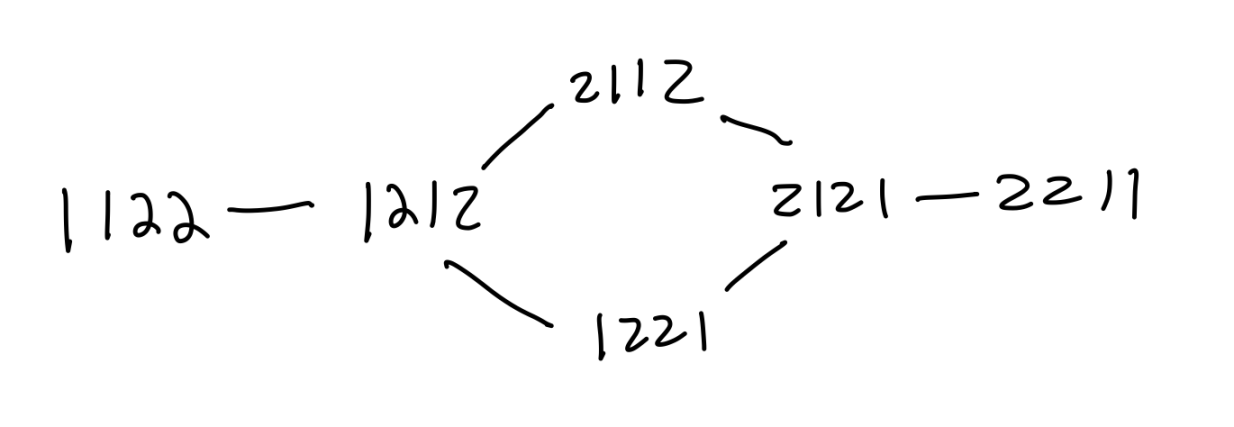
\includegraphics[scale=.25]{image.png}

\begin{itemize}
    \item No path that covers all nodes \pause
    \item Luckily, permuting distinct sets is usually what happens most often in practice
\end{itemize}
\end{frame}

\begin{frame}{Intuition}
\begin{itemize}
    \item Consider trying to find the permutations when $n=4$: $\{1,2,3,4\}$ \pause
    \item What if you took the permutations of $n=3$, and inserted $4$ into every position? \pause
\end{itemize}
\begin{table}[]
\begin{tabular}{llllll}
123 & 132 & 312 & 321 & 231 & 213 \pause \\
\end{tabular}
\end{table}
\begin{itemize}
    \item Inserting \textcolor{sigma@mainblue}{4}'s in a snaking pattern by column, you have your sequence of permutations
\end{itemize}
\begin{table}[]
\begin{tabular}{llllll}
123\textcolor{sigma@mainblue}{4} & 132\textcolor{sigma@mainblue}{4} & 312\textcolor{sigma@mainblue}{4} & 321\textcolor{sigma@mainblue}{4} & 231\textcolor{sigma@mainblue}{4} & 213\textcolor{sigma@mainblue}{4} \pause \\
12\textcolor{sigma@mainblue}{4}3 & 13\textcolor{sigma@mainblue}{4}2 & 31\textcolor{sigma@mainblue}{4}2 & 32\textcolor{sigma@mainblue}{4}1 & 23\textcolor{sigma@mainblue}{4}1 & 21\textcolor{sigma@mainblue}{4}3 \pause \\
1\textcolor{sigma@mainblue}{4}23 & 1\textcolor{sigma@mainblue}{4}32 & 3\textcolor{sigma@mainblue}{4}12 & 3\textcolor{sigma@mainblue}{4}21 & 2\textcolor{sigma@mainblue}{4}31 & 2\textcolor{sigma@mainblue}{4}13 \\
\textcolor{sigma@mainblue}{4}123 & \textcolor{sigma@mainblue}{4}132 & \textcolor{sigma@mainblue}{4}312 & \textcolor{sigma@mainblue}{4}321 & \textcolor{sigma@mainblue}{4}231 & \textcolor{sigma@mainblue}{4}213
\end{tabular}
\end{table}
\end{frame}

\begin{frame}{Algorithm P}
\begin{nalgo}[0.95]
\textul{\textbf{\textsc{AlgorithmP}}$(S[a_0, \dots, a_n])$}:
\\\label{}  $C[1..n] \gets 0, O[1..n] \gets 1$
\\\label{}  \textbf{while} \textsc{True}:\+
\\\label{}      \textsc{print}$(S)$
\\\label{}      $j \gets n, s \gets 0$
\\\label{}      \textbf{A:}~~$q \gets C[j] + O[j]$\+
\\\label{}          \textbf{if} $q < 0$: goto \textbf{D}
\\\label{}          \textbf{if} $q = j$: goto \textbf{B}
\\\label{}          \textsc{swap}$(S, j-C[j]+s, j-q+s)$
\\\label{}          $C[j] \gets q$ 
\\\label{}          continue\-
\\\label{}      \textbf{B:}~~\textbf{if} $j=1$:\+\+
\\\label{}              break\-
\\\label{}          $s \gets s+1$\-
\\\label{}    \textbf{D:}~~$O[j] \gets -O[j], j \gets j-1$\+
\\\label{}      goto \textbf{A}
\end{nalgo}
\end{frame}

\begin{frame}{}
\begin{minipage}[c]{0.6\textwidth}
\begin{nalgo}
\textul{\textbf{\textsc{AlgorithmP}}$(S[a_0, \dots, a_n])$}:
\\\label{}  $C[1..n] \gets 0, O[1..n] \gets 1$
\\\label{}  \textbf{while} \textsc{True}:\+
\\\label{}      \textsc{print}$(S)$
\\\label{}      {\color{lightgray}$j \gets n, s \gets 0$}
\\\label{}      {\color{lightgray}\textbf{A:}~~$q \gets C[j] + O[j]$\+}
\\\label{}          {\color{lightgray}\textbf{if} $q < 0$: goto \textbf{D}}
\\\label{}          {\color{lightgray}\textbf{if} $q = j$: goto \textbf{B}}
\\\label{}          {\color{lightgray}\textsc{swap}$(S, j-C[j]+s, j-q+s)$}
\\\label{}          {\color{lightgray}$C[j] \gets q$} 
\\\label{}          {\color{lightgray}continue\-}
\\\label{}      {\color{lightgray}\textbf{B:}~~\textbf{if} $j=1$:\+\+}
\\\label{}              {\color{lightgray}break\-}
\\\label{}          {\color{lightgray}$s \gets s+1$\-}
\\\label{}    {\color{lightgray}\textbf{D:}~~$O[j] \gets -O[j], j \gets j-1$\+}
\\\label{}      {\color{lightgray}goto \textbf{A}}
\end{nalgo}
\end{minipage}
\begin{minipage}[c]{0.35\textwidth}
\begin{itemize}
    \item We initialize $C$, which tracks inversions, i.e. the distance $a_k$ is from $k$ in later iterations \pause
    \item We initialize $O$ which tracks which direction values in $C$ have changed (left or right) \pause
    \item Every iteration, we print out a permutation
\end{itemize}
\end{minipage}
\end{frame}

\begin{frame}{}
\begin{minipage}[c]{0.6\textwidth}
\begin{nalgo}
\textul{\textbf{\textsc{AlgorithmP}}$(S[a_0, \dots, a_n])$}:
\\\label{}  {\color{lightgray}$C[1..n] \gets 0, O[1..n] \gets 1$}
\\\label{}  {\color{lightgray}\textbf{while} \textsc{True}:\+}
\\\label{}      {\color{lightgray}\textsc{print}$(S)$}
\\\label{}      $j \gets n, s \gets 0$
\\\label{}      {\color{lightgray}\textbf{A:}~~$q \gets C[j] + O[j]$\+}
\\\label{}          {\color{lightgray}\textbf{if} $q < 0$: goto \textbf{D}}
\\\label{}          {\color{lightgray}\textbf{if} $q = j$: goto \textbf{B}}
\\\label{}          {\color{lightgray}\textsc{swap}$(S, j-C[j]+s, j-q+s)$}
\\\label{}          {\color{lightgray}$C[j] \gets q$} 
\\\label{}          {\color{lightgray}continue\-}
\\\label{}      {\color{lightgray}\textbf{B:}~~\textbf{if} $j=1$:\+\+}
\\\label{}              {\color{lightgray}break\-}
\\\label{}          {\color{lightgray}$s \gets s+1$\-}
\\\label{}    {\color{lightgray}\textbf{D:}~~$O[j] \gets -O[j], j \gets j-1$\+}
\\\label{}      {\color{lightgray}goto \textbf{A}}
\end{nalgo}
\end{minipage}
\begin{minipage}[c]{0.35\textwidth}
\begin{itemize}
    \item We track the coordinate $j$ where $C[j]$ is about to change, such that $0\leq C[j] < j$ for all $j$ \pause
    \item $s$ tracks the number of indices $k$ such that $C[k] = k-1$ where $k > j$
\end{itemize}
\end{minipage}
\end{frame}

\begin{frame}{}
\begin{minipage}[c]{0.6\textwidth}
\begin{nalgo}
\textul{\textbf{\textsc{AlgorithmP}}$(S[a_0, \dots, a_n])$}:
\\\label{}  {\color{lightgray}$C[1..n] \gets 0, O[1..n] \gets 1$}
\\\label{}  {\color{lightgray}\textbf{while} \textsc{True}:\+}
\\\label{}      {\color{lightgray}\textsc{print}$(S)$}
\\\label{}      {\color{lightgray}$j \gets n, s \gets 0$}
\\\label{}      \textbf{A:}~~$q \gets C[j] + O[j]$\+
\\\label{}          \textbf{if} $q < 0$: goto \textbf{D}
\\\label{}          \textbf{if} $q = j$: goto \textbf{B}
\\\label{}          \textsc{swap}$(S, j-C[j]+s, j-q+s)$
\\\label{}          $C[j] \gets q$
\\\label{}          continue\-
\\\label{}      {\color{lightgray}\textbf{B:}~~\textbf{if} $j=1$:\+\+}
\\\label{}              {\color{lightgray}break\-}
\\\label{}          {\color{lightgray}$s \gets s+1$\-}
\\\label{}    {\color{lightgray}\textbf{D:}~~$O[j] \gets -O[j], j \gets j-1$\+}
\\\label{}      {\color{lightgray}goto \textbf{A}}
\end{nalgo}
\end{minipage}
\begin{minipage}[c]{0.35\textwidth}
\begin{itemize}
    \item We determine $q$ from $C$ and $O$. If $q$ is less than 0, we switch directions at \textbf{D}. If $q=j$ we need to increase $s$ and switch directions, if possible \pause
    \item Otherwise, we swap the two relative locations within $S$ and print out a permutation
\end{itemize}
\end{minipage}
\end{frame}

\begin{frame}{}
\begin{minipage}[c]{0.6\textwidth}
\begin{nalgo}
\textul{\textbf{\textsc{AlgorithmP}}$(S[a_0, \dots, a_n])$}:
\\\label{}  {\color{lightgray}$C[1..n] \gets 0, O[1..n] \gets 1$}
\\\label{}  {\color{lightgray}\textbf{while} \textsc{True}:\+}
\\\label{}      {\color{lightgray}\textsc{print}$(S)$}
\\\label{}      {\color{lightgray}$j \gets n, s \gets 0$}
\\\label{}      {\color{lightgray}\textbf{A:}~~$q \gets C[j] + O[j]$\+}
\\\label{}          {\color{lightgray}\textbf{if} $q < 0$: goto \textbf{D}}
\\\label{}          {\color{lightgray}\textbf{if} $q = j$: goto \textbf{B}}
\\\label{}          {\color{lightgray}\textsc{swap}$(S, j-C[j]+s, j-q+s)$}
\\\label{}          {\color{lightgray}$C[j] \gets q$} 
\\\label{}          {\color{lightgray}continue\-}
\\\label{}      \textbf{B:}~~\textbf{if} $j=1$:\+\+
\\\label{}              break\-
\\\label{}          $s \gets s+1$\-
\\\label{}    \textbf{D:}~~$O[j] \gets -O[j], j \gets j-1$\+
\\\label{}      goto \textbf{A}
\end{nalgo}
\end{minipage}
\begin{minipage}[c]{0.35\textwidth}
\begin{itemize}
    \item If we need to increase $s$, we check if $j=1$ and terminate, then we move to \textbf{D} to switch directions \pause
    \item \textbf{D} switches the direction stored in $O$ and decrements $j$ and returns to \textbf{A} to try again
\end{itemize}
\end{minipage}
\end{frame}

% \begin{frame}{Algorithm P}
% \begin{algo}
% $C[1..n] \gets 0, O[1..n] \gets 1$ \\
% \textbf{while} \textsc{True}:\+ \\
%     \textsc{print}$(S)$
% \end{algo}
% \begin{itemize}
%     \item We initialize $C$, which tracks inversions, i.e. the distance $a_k$ is from $k$ in later iterations. \pause
%     \item We initialize $O$ which tracks which direction values in $C$ have changed (left or right). \pause
%     \item Every iteration, we print out a permutation.
% \end{itemize}
% \end{frame}

% \begin{frame}{Algorithm P}
% \begin{algo}
%     $j \gets n, s \gets 0$
% \end{algo}
% \begin{itemize}
%     \item We track the coordinate $j$ where $C[j]$ is about to change, such that $0\leq C[j] < j$ for all $j$.
%     \item $s$ tracks the number of indices $k$ such that $C[k] = k-1$ where $k > j$.
% \end{itemize}
% \end{frame}

% \begin{frame}{Algorithm P}
% \begin{algo}
%         \textbf{A:}~~$q \gets C[j] + O[j]$\+
% \\          ~~~\textbf{if} $q < 0$: goto \textbf{D}
% \\          ~~~\textbf{if} $q = j$: goto \textbf{B}
% \\          ~~~\textsc{swap}$(S, j-C[j]+s, j-q+s)$
% \\          ~~~continue\-
% \end{algo}
% \begin{itemize}
%     \item We determine $q$ from $C$ and $O$. If $q$ is less than 0, we switch directions at \textbf{D}. If $q=j$ we need to increase $s$ and switch directions, if possible. \pause
%     \item Otherwise, we swap the two relative locations within $S$ and print out a permutation.
% \end{itemize}
% \end{frame}

% \begin{frame}{Algorithm P}
% \begin{algo}
%         \textbf{B:}~~\textbf{if} $j=1$:\+\+
% \\              break\-
% \\          ~~~$s \gets s+1$\-
% \\    \textbf{D:}~~$O[j] \gets -O[j], j \gets j-1$\+
% \\      ~~~goto \textbf{A}
% \end{algo}
% \begin{itemize}
%     \item If we need to increase $s$, we check if $j=1$ and terminate, then we move to \textbf{D} to switch directions \pause
%     \item \textbf{D} switches the direction stored in $O$ and decrements $j$ and returns to \textbf{A} to try again.
% \end{itemize}
% \end{frame}

\begin{frame}{}
      \begin{center}
    {\color{sigma@mainblue} \LARGE Questions?}
  \end{center}
\end{frame}

% \begin{frame}{Questions!}
% \begin{itemize}
%     \item What is (crudely) the runtime of this algorithm?
%     \item What is the runtime of the delay between permutations? 
% \end{itemize}
% \end{frame}

\section{Conclusion}
\frame{\sectionpage}

\begin{frame}
Other interesting algorithms from this chapter:
\begin{itemize}
    \item Algorithm T: Extends Algorithm P to output an array of transitions, to reuse generating permutations in constant time \pause
    \item Algorithm G: A generalized approach to producing permutations when given a group of subsets of $S$ \pause
    \item Algorithm X: An extension to Algorithm L to generate permutations satisfying some conditions efficiently
    \begin{itemize}
        \item It does this by maintaining a linked list of available elements
        \item This is not Algorithm X from last week
    \end{itemize}
\end{itemize}
\end{frame}

\font\eightss=cmssq8
\font\eightssi=cmssqi8
\newcommand\quoteAuthorDate[3]{\begingroup
  \baselineskip 10pt
  \parfillskip 0pt
  \interlinepenalty 10000 % not needed in example
  \leftskip 0pt plus 40pc minus \parindent
  \let\rm=\eightss
  \let\sl=\eightssi
  \everypar{\sl}#1\par
  \nobreak\smallskip
  \noindent\rm--- #2\unskip\enspace(#3)\par
  \endgroup}

\begin{frame}
    \begin{center}
        \item \quoteAuthorDate{A permutation on the ten decimal digits is simply a 10 digit decimal number in which all digits are distinct. Hence all we need to do is to produce all 10 digit numbers and select only those who digits are distinct. Isn't it wonderful how high speed computing saves us from the drudgery of thinking! We simply program $k+1 \to k$ and examine the digits of $k$ for undesirable equalities. This gives us the permutations in dictionary order too! \newline On second sober thought ... we do need to think of something else.}{D. H. LEHMER}{\color{sigma@mainblue}1957}
    \end{center}
\end{frame}

% Remove this slide if you came up with all the material yourself
\begin{frame}{Bibliography}
    \bibliography{refs}
    \bibliographystyle{alpha}
\end{frame}

\end{document}